\documentclass{article}

\usepackage{hyperref}
%\hypersetup{colorlinks, %
%	citecolor=black,%
%	filecolor=black,%
%	linkcolor=black,%
%	urlcolor=black,%
%	pdftex}	
\usepackage{graphicx}
\usepackage{tikz}
\usepackage{amssymb,amsmath}
\usepackage{float}
\newcommand{\email}[1]{\texttt{#1}}
\newcommand{\gmat}{GMAT}
\newcommand{\vim}{\href{http://www.vim.org} {www.vim.org} }

\title{\gmat{} Maths Grinds}
\author{Conor Gilmer $<$\href{mailto:conor.gilmer@gmail.com}{conor.gilmer@gmail.com}$>$}


\begin{document}

\section{Probability}
Probability of an event is the number of results over the total number of possible results.
\begin{equation}
P(E) = \frac{Number\;of\;outcomes}{Total\;number\;of\;possible}
\end{equation}
\textbf{e.g}
If you throw a dice twice what are the chances (probability) of 1 side being shown.

$P(E) = \frac{2}{6} = \frac{1}{3}$

This often described as a $1$ in $3$ chance of occurring.

\subsection{Probability Arithmetic}
Rule of thumb in combining probability is if you have two events, and you want to know the probability of 
\begin{itemize}
\item Probability of Event A \textbf{AND} Event B =  $P(A) * P(B)$
\item Probability of Event A \textbf{OR} Event B =  $P(A) + P(B)$
\item Probability of an Event E \textbf{NOT} occurring $P(NOT E) = P(\overline{E}) = 1 - P(E)$
\end{itemize}

\textbf{e.g}
If you throw two dice (Dice A and Dice B) at the same time, what are the chances (probability) of the number 6 been shown on (1) both the dice A AND dice B, (2) Probability or either dice A OR dice B being the number 6 and (3) chances of the number 6 NOT landing on both dice A AND dice B.

(1)

$\\P(A\;AND\;B) = P(A) * P(B) \\
P(A\;AND\;B) = \frac{1}{6} * \frac{1}{6} \\
P(A\;AND\;B) = \frac{1 * 1}{6 * 6} = \frac{1}{36}
$

(2)

$\\P(A\;OR\;B) = P(A) + P(B) \\
P(A\;OR\;B) = \frac{1}{6} + \frac{1}{6} \\
P(A\;OR\;B) = \frac{1 + 1}{6} = \frac{2}{6} = \frac{1}{3}
$

(3)

$\\NOT\;(P(A\;AND\;B)) = 1 - (P(A) * P(B)) \\
NOT \;P(A\;AND\;B) = 1 - (\frac{1}{6} * \frac{1}{6}) \\
NOT \; P(A\;AND\;B) = 1 -(\frac{1 * 1}{6 * 6}) = 1 - (\frac{1}{36}) = \frac{36-35}{36} = \frac{35}{36}
$

\newpage
\section{Sets}
A Set is a collection of objects, in mathematics it is generally a collection of numbers but could be other objects.
\begin{itemize}
\item \textbf{Union} A Union B is all the contents of sets A and B. $A \cup B$
\item \textbf{Intersection} A intersection B is the contents which are common to A and B. $A \cap B$ 
\item \textbf{NOT} A NOT B is contents of set A which is not in set B. $A - B$ %or $A \cap \overline{B}$ 
\end{itemize}
\subsection{Venn Diagram}
Sets can be represented diagramatically using Venn Diagrams.

\textbf{A Union B}
\begin{center}
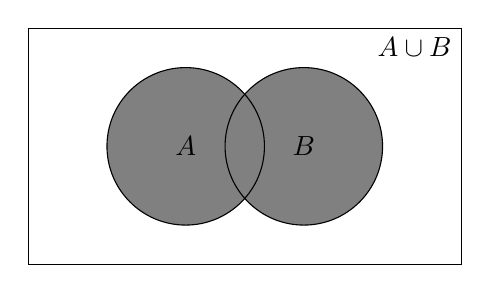
\begin{tikzpicture}
\draw (-2,-1.5) rectangle (3.5,1.5) node[below left]{$A \cup B$};
\fill[gray] (0,0) circle (1cm);
\fill[gray] (1.5,0) circle (1cm);
\draw (0,0) circle (1cm) node {$A$};
\draw (1.5,0) circle (1cm) node {$B$};
\end{tikzpicture}
\end{center}

\textbf{A Intersection B}
\begin{center}
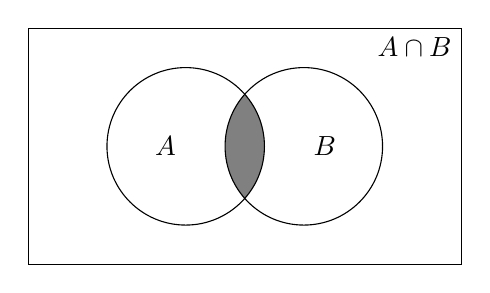
\begin{tikzpicture}
\draw (-2,-1.5) rectangle (3.5,1.5) node[below left]{$A \cap B$};
\begin{scope} % start of clip scope
\clip (0,0) circle (1cm);
\fill[gray] (1.5,0) circle (1cm);
\end{scope} % end of clip scope
\draw (0,0) circle (1cm) node[left] {$A$};
\draw (1.5,0) circle (1cm) node[right] {$B$};
\end{tikzpicture}
\end{center}


\textbf{A Intersection B NOT C}
\def \setA{ (0,0) circle (1cm) }
\def \setB{ (1.5,0) circle (1cm) }
\def \setC{ (60:1.5) circle (1cm) }
\def \setU{ (-2, -1.5) rectangle (3.5, 2.75) }
\begin{center}
\begin{tikzpicture}
\draw \setU node[below left]{$A \cap B \cap \overline{\rm C}$};
\begin{scope}
\clip \setA;
\fill[gray] \setB;
\end{scope}
\begin{scope}
\clip \setA;
\clip \setB;
\fill[white] \setC;
\end{scope}
\draw \setA node[left] {$A$};
\draw \setB node[right] {$B$};
\draw \setC node {$C$};
\end{tikzpicture}
\end{center}




\end{document}